\documentclass{article}
\usepackage[T1]{fontenc}
\usepackage[polish]{babel}
\usepackage[utf8]{inputenc}
\usepackage{graphicx} % Required for inserting images

\title{MOwNiT - Laboratorium 6:\\
Układy równań – metody bezpośrednie}
\author{Wojciech Dąbek}
\date{30 kwietnia 2024}

\begin{document}

\maketitle

\section{Treść zadań}

Napisz program, który:
\begin{enumerate}
    \item Jako parametr pobiera rozmiar układu równań \textit{n}
    \item Generuje macierz układu \(A(n \times n)\) i wektor wyrazów wolnych \(b(n)\)
    \item Rozwiązuje układ równań \(Ax = b\) na trzy sposoby:
    \begin{itemize}
        \item poprzez dekompozycję LU macierzy \(A: A = LU\)
        \item poprzez odwrócenie macierzy \(A: x = A^{-1} b\),\\
        sprawdzić czy \(A A^{-1} = I\) i \(A^{-1} A = I\) (macierz jednostkowa)
        \item poprzez dekompozycję QR macierzy \(A: A = QR\)
    \end{itemize}
    \item Sprawdzi poprawność rozwiązania (tj. czy \(Ax = b\))
    \item Zmierzy całkowity czas rozwiązania układu
    \item Porównać czasy z trzech sposobów: poprzez dekompozycję LU, poprzez odwrócenie macierzy i poprzez dekompozycję QR.
\end{enumerate}

\noindent
Narysuj wykres zależności całkowitego czasu rozwiązywania układu (LU, QR, odwrócenie macierzy) od rozmiaru układu równań. Wykonaj pomiary dla 5 wartości z przedziału od 10 do 100.

\vspace{5mm}
\noindent
\textit{Uwaga: można się posłużyć funkcjami z biblioteki numerycznej dla danego języka programowania.}

\newpage

\section{Rozwiązanie}
Program do tego zadania napisałem w języku Python posługując się biblioteką numeryczną NumPy. Plik z kodem \verb|eq_solver.py| jest dołączony obok tego sprawozdania.

\vspace{5mm}
\noindent
Wykres zależności całkowitego czasu rozwiązywania układu od rozmiaru układu równań zrealizowałem w programie MS Excel. Pomiary 5 wybranych wartości czasu obliczeń wypisanych przez mój program wyglądają następująco:
\begin{figure}[h]
    \centering
    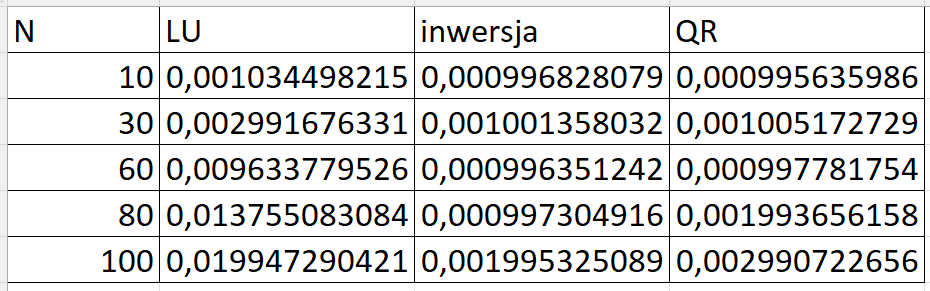
\includegraphics[width=\linewidth]{tabela.png}
\end{figure}

\noindent
A wykres dla powyższych danych:
\begin{figure}[h]
    \centering
    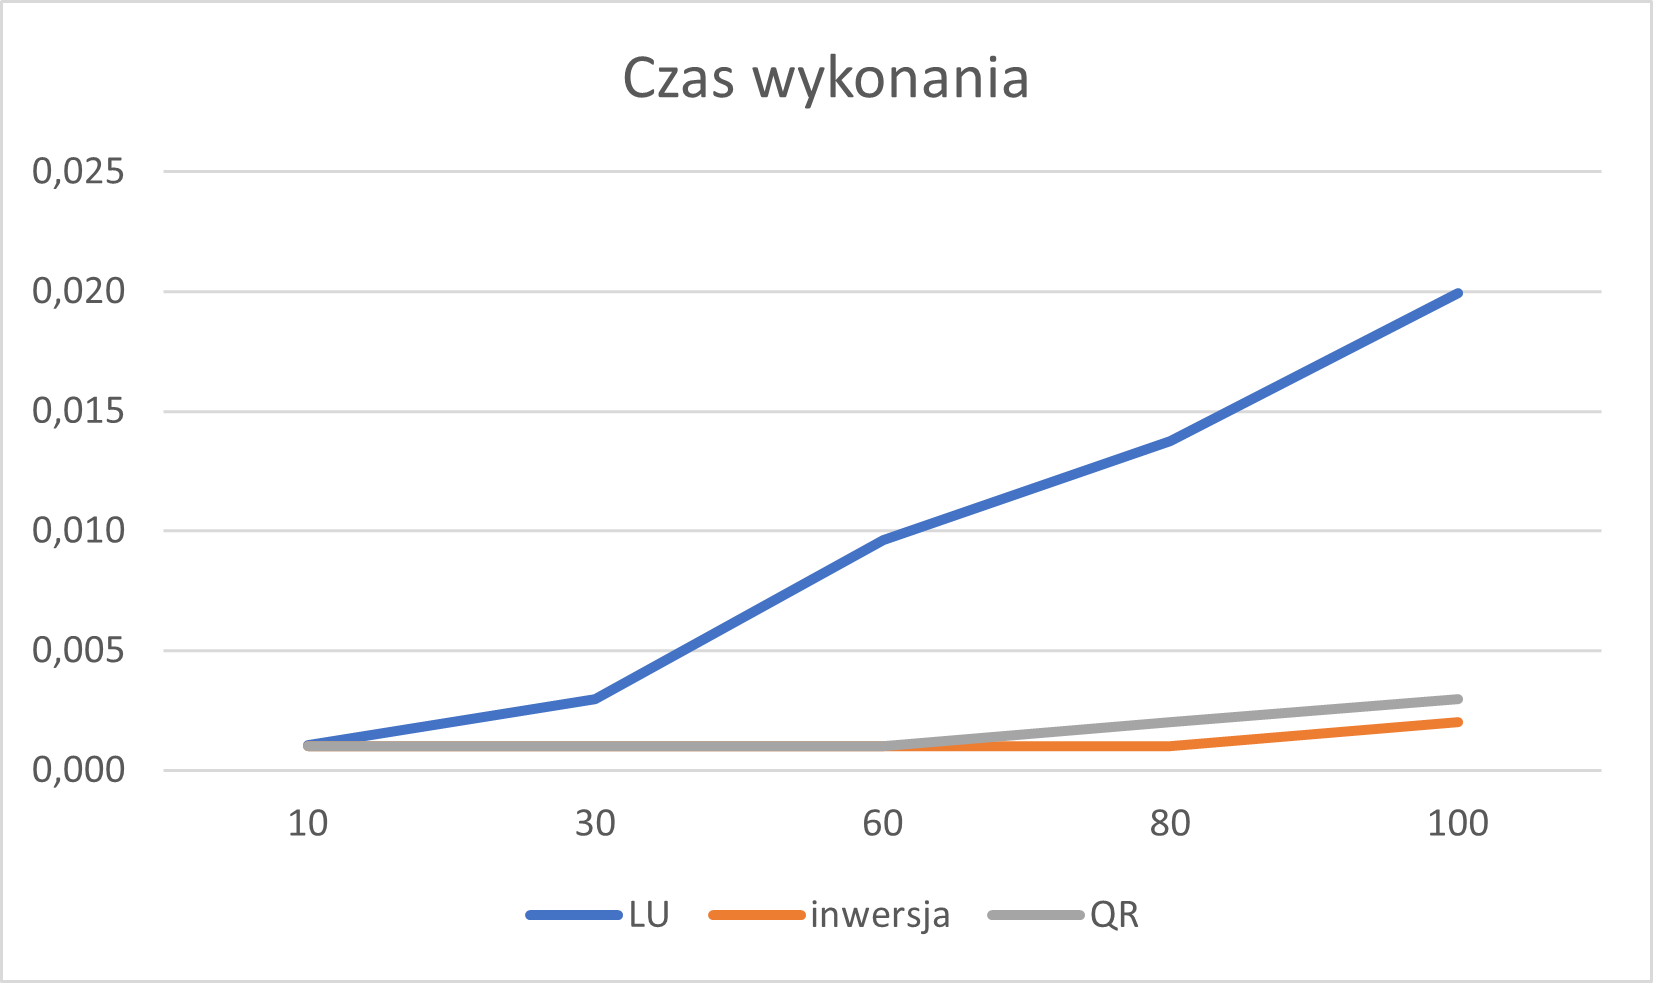
\includegraphics[width=\linewidth]{wykres.png}
\end{figure}

\newpage

\section{Wnioski}
Wyraźnie najgorszy czas zmierzony został dla metody rozkładu LU, dwie pozostałe są podobnie szybkie. Wynika to przede wszystkim z tego, że algorytm rozkładu LU napisałem w niemal czystym (i wolnym) Pythonie. Pozostałe metody opierają się w większym stopniu o możliwości biblioteki numerycznej NumPy, która dzięki byciu opartą o język C jest bardzo wydajna.\\
Co więcej, zadane tylko 5 pomiarów na takim przedziale może nie oddawać dobrze różnic między wydajnością podejść z inwersją i rozkładem QR.

\section{Bibliografia}
https://pl.wikipedia.org/wiki/Metoda\_LU\\
https://pl.wikipedia.org/wiki/Rozkład\_QR\\
https://numpy.org/doc/stable/

\end{document}
